\documentclass[../AnalisideiRequisiti.tex]{subfiles}

\begin{document}
	
\chapter{Descrizione generale}

\section{Obiettivo del prodotto}

Lo scopo del progetto consiste nel creare un applicativo software di supporto allo sviluppo di \glossario{Speect}{Speect}. L’applicazione da creare è una interfaccia grafica che aiuti i programmatori nello sviluppo dei plug-in per Speect. Nell’interfaccia utente si devono poter visualizzare e modificare i grafi delle \glossario{utterance}{utterance} di Speect. 


\section{Funzioni del prodotto}
L’interfaccia grafica permetterà di:
\begin{itemize}
	\item{} Caricare i \glossario{file .json}{file .json} utili all’inizializzazione di Speect;
	\item{} Mostrare i grafi delle varie utterance;
	\item{} Aggiungere, modificare e eliminare gli archi dei nodi;
	\item{} Modificare dei campi dei nodi;
	\item{} Disporre graficamente i nodi per permettere una lettura semplificata;
	\item{} Restituire il file audio generato da Speect;
	\item{} Stampare i grafi su schermo;
	\item{} Visualizzare passo passo i grafi delle varie utterance in modo sequenziale, cioè l’utente potrà decidere quando eseguire e visualizzare il grafo della successiva utterance.	
\end{itemize}


\section{Caratteristiche degli utenti}
Il software si rivolge a programmatori esperti che si occupano di sviluppare plug-in per Speect. Per poter fruire correttamente del prodotto, l'utente deve dunque possedere un'approfondita conoscenza di Speect e delle sue componenti.

\section{Piattaforma di esecuzione}
Sarà garantita l'esecuzione del software su tutte le macchine desktop e laptop con sistema operativo Linux su cui siano presenti \glossario{CMAKE}{CMAKE}, \glossario{GCC}{GCC} e le librerie di \glossario{QT}{QT}. Verranno comunque utilizzate tecnologie presenti anche su sistemi Windows, il che renderà possibile la compilazione anche in questo ambiente. Per quest'ultima piattaforma, tuttavia, non verrà fornito un manuale di installazione.

\section{Vincoli generali}
Il software realizzato deve fare uso della tecnologia Speect offerta dalla Proponente, e deve essere utilizzabile su sistema operativo Linux Ubuntu 16.04 \glossario{LTS}{LTS}.
	

\chapter{Interfaccia Grafica}

\section{Introduzione}

Questo capitolo ha lo scopo di presentare, in linea generale, il funzionamento dell'interfaccia grafica. Le interfacce proposte nelle immagini riportate nelle sezioni seguenti non rappresentano un progetto di implementazione definitivo, bensì una linea guida per una miglior comprensione delle varie funzionalità dell'applicazione. L'estetica del prodotto concluso potrebbe dunque differire dalle immagini riportate in questo documento. Si fa inoltre notare che le istruzioni che seguono non intendono essere in alcun modo una guida all'utilizzo dell'applicazione.


	\section{Schermata principale}
		\begin{figure}[htp]
			\caption{Esempio pagina principale}
			\centering
			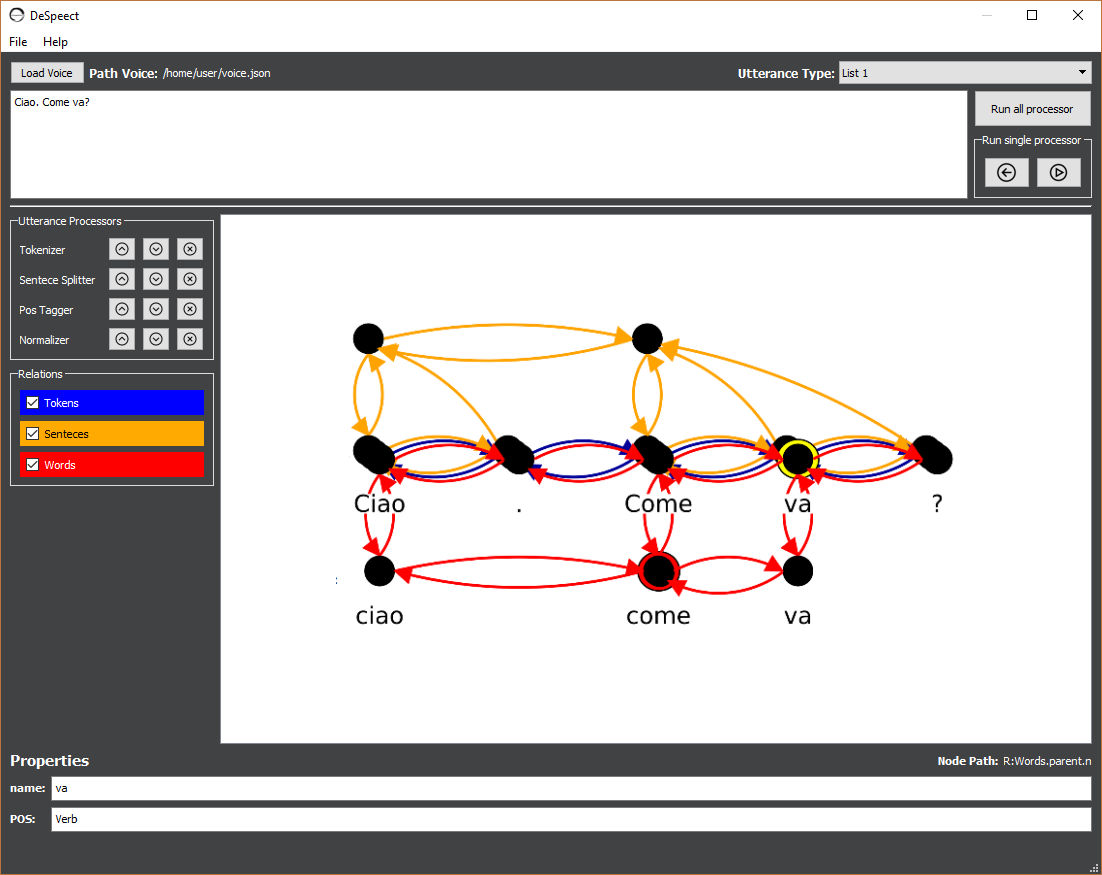
\includegraphics[width=\textwidth]{../img/paginainiziale.png}
			\label{fig:GUI}
		\end{figure}	
		Nell'interfaccia grafica saranno presenti due pulsanti per caricare il \glossario{file Voice JSon}{file voice .json}: uno in alto a sinistra etichettato "Load Voice" (vedi \ref{fig:GUI}) e uno di nome "Load Voice JSon" all'interno della voce "File" nella barra del menu (vedi \ref{fig:menufile}).
		 A seguito del caricamento del file Voice Json il menù a tendina "Utterance Type" (vedi \ref{fig:GUI} in alto a destra) viene popolato con l'elenco delle varie \glossario{utterance type}{utterance type} contenute nel file stesso. 
		 Una volta selezionata la \glossario{utterance type}{utterance type} desiderata, il programma riempie l'elenco "Utterance Processor" (vedi \ref{fig:GUI} sulla sinistra appena al di sotto della linea orizzontale che separa la parte superiore dell'applicazione da quella inferiore contenente anche la stampa del grafo) con una lista di \glossario{utterance processor}{utterance processor} contenuti nella utterance type selezionata. 
		 In seguito, l'utente può compilare l'area di testo sottostante il pulsante "Load Voice" (vedi \ref{fig:GUI}) con il testo che desidera far elaborare a \glossario{Speect}{Speect}.
		 Proseguendo verso destra, nella figura \ref{fig:GUI}, l'utente ha la possibilità di eseguire tutti gli \glossario{utterance processor}{utterance processor} contenuti nella utterance type premendo il pulsante "Run all processor" (vedi \ref{fig:GUI}), in alternativa, può eseguirli sequenzialmente uno alla volta con la possibilità di tornare al passo precedente (vedi pulsanti contenuti nell'area nominata "Run single processor" \ref{fig:GUI}).  Man mano che gli utterance processor vengono eseguiti, nell'area centrale bianca (vedi \ref{fig:GUI}) viene disegnato il \glossario{grafo HRG}{grafo HRG}. Nella sezione degli utterance processor (vedi \ref{fig:GUI}) l'utente avrà la possibilità di:
		\begin{itemize}
			\item{}modificare l'ordine di esecuzione delle utterance agendo sulle freccie a lato della singola utterance processor;
			\item{}rimuovere una determinata utterance processor dall'elenco e quindi dalla utterance type.
		\end{itemize}
		Nel riquadro denominato "Relations" l'utente ha la possibilità di decidere quali relazioni, del grafo HRG, visualizzare. Cliccando un nodo del grafo HRG l'utente lo evidenza con un cerchio di colore giallo e può visualizzare, nella parte inferiore dell'interfaccia grafica, le sue proprietà, tra cui il percorso del nodo.
	\begin{figure}[htp]
	\caption{Esempio voce File nella barra del menu}
	\centering
	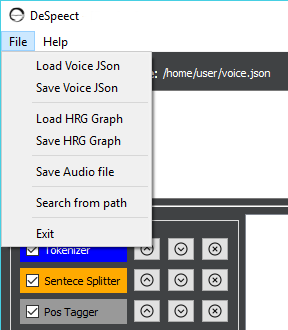
\includegraphics[]{../img/menu-file.png}
	\label{fig:menufile}
\end{figure}
	\\ Attraverso la voce "File" della barra del menu (vedi \ref{fig:menufile}) l'utente ha accesso alle seguenti funzioni:
	 	
		\begin{itemize}
			\item \textbf{Load Voice JSon:} caricamento del file di inizializzazione di Speect;
			\item \textbf{Save Voice JSon:} salvataggio del file di inizializzazione di Speect;
			\item \textbf{Load HRG Graph:} caricamento e visualizzazione nell'area apposita di un grafo HRG;
			\item \textbf{Save HRG Graph:} salvataggio dello stato di un grafo HRG;
			\item \textbf{Save Audio file:} salvataggio del file audio prodotto dall'esecuzione di Speect;
			\item \textbf{Search from path:} evidenziazione del nodo nel grafo HRG e conseguente visualizzazione delle sue proprietà;
			\item \textbf{Exit:} Uscita dall'applicazione.
		\end{itemize}
		 Attraverso la voce "Help" della barra del menu (vedi \ref{fig:menuhelp}) l'utente ha accesso alle seguenti funzioni:
		\begin{itemize}
			\item \textbf{Manual:} visualizzazione del manuale utente;
			\item \textbf{Licence:} visualizzazione della licenza del prodotto;
			
		\end{itemize}
	
		\begin{figure}[htp]
			\caption{Esempio voce Help nella barra di menu}
			\centering
			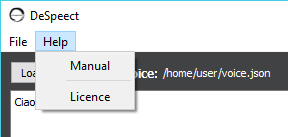
\includegraphics[]{../img/menu-help.png}
			\label{fig:menuhelp}
		\end{figure}
		
	\section{Schermata caricamento file}
	
		Mediante questa schermata (\ref{fig:filebrowser-load}) l'utente può navigare attraverso il \glossario{file system}{file system} e selezionare il file che desidera aprire. 
		Nell'area centrale bianca vengono visualizzati i file e le cartelle del percorso specificato nella barra "Path". Facendo doppio clic su una cartella, contenuta nel blocco centrale, verrà cambiato il percorso del "Path" e quindi verrà visualizzato il suo contenuto.
		Il primo pulsante in alto a sinistra è utilizzato per raggiungere la directory padre e visualizzarne il contenuto nell'area dedicata.
		Il pulsante in alto a destra, denotato dall'icona rappresentate una cartella, permette all'utente di creare una nuova cartella nel percorso indicato nella barra "Path". 
		Una volta individuato il file da aprire l'utente ha a disposizione i seguenti tre modi per aprirlo:
		\begin{enumerate}
			\item{} Doppio clic sopra il file;
			\item{} Un clic sopra il file seguito dalla pressione del pulsante "Open";
			\item{} Scrittura del nome del file, compreso di estensione, seguito dalla pressione del pulsante "Open".
		\end{enumerate}
		\begin{figure}[htp]
			\caption{Esempio finestra caricamento file}
			\centering
			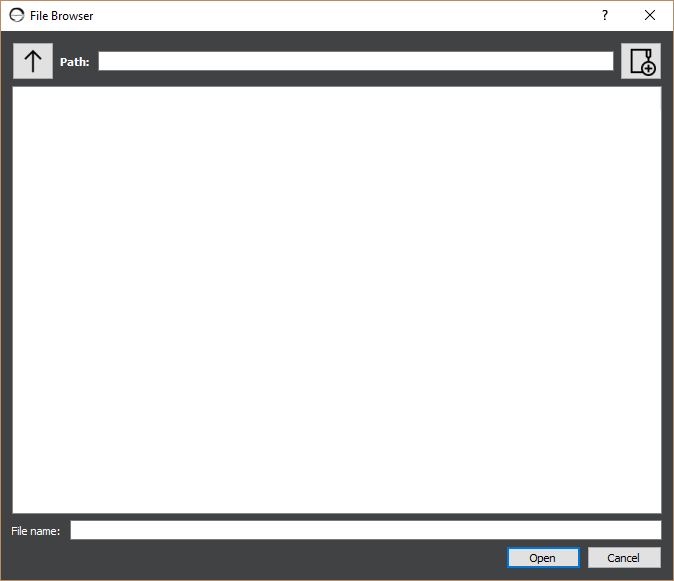
\includegraphics[width=\textwidth]{../img/filebrowser-load.png}
			\label{fig:filebrowser-load}
		\end{figure}

	\section{Schermata salvataggio file}
	
	
		Mediante questa schermata (\ref{fig:filebrowser-save}) l'utente ha la possibilità di navigare attraverso il \glossario{file system}{file system} e di posizionarsi all'interno della cartella nella quale vuole salvare il file.
		Nell'area centrale bianca vengono visualizzati i file e le cartelle del percorso specificato nella barra "Path". Facendo doppio clic su una cartella, contenuta nel blocco centrale, verrà cambiato il percorso del "Path" e quindi verrà visualizzato il suo contenuto.
		Il primo pulsante in alto a sinistra è utilizzato per raggiungere la directory padre e visualizzarne il contenuto nell'area dedicata.
		Il pulsante in alto a destra, invece permette all'utente di creare una nuova cartella nel percorso indicato nella barra "Path". 
		Una volta individuato il punto in cui salvare il file è necessario attenersi alla seguente procedura per salvarlo:
		\begin{enumerate}
			\item{} Scrivere il nome del file nell'apposito campo senza riportare l'estensione;
			\item{} Selezionare l'estensione del file;
			\item{} Premere il pulsante "Save".
		\end{enumerate}
	\begin{figure}[htp]
			\caption{Esempio finestra salvataggio file}
			\centering
			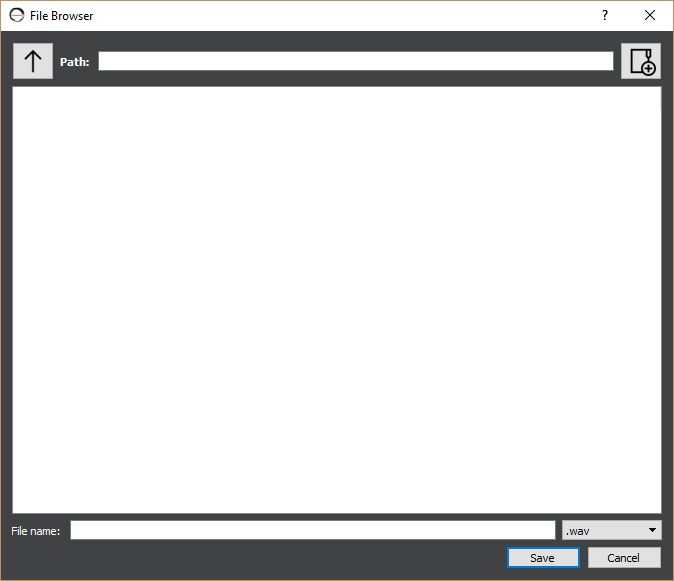
\includegraphics[width=\textwidth]{../img/filebrowser-save.png}
			\label{fig:filebrowser-save}
		\end{figure}

\end{document}